% !TEX encoding = UTF-8
% !TEX TS-program = pdflatex
% !TEX root = ../tesi.tex

%**************************************************************
\chapter{Il contesto aziendale}
\label{cap:processi-metodologie}
%**************************************************************

%**************************************************************
\section{L'azienda: \textbf{\azienda}}
\textbf{\azienda} nasce nel 2013 come azienda focalizzata nello sviluppo di soluzioni basate sui profili comportamentali, cioè l'analisi dei comportamenti abituali di determinati utenti, in ambito di sicurezza ed antifrode. Nel 2014 ha rilasciato le prime soluzioni sulla protezione ed analisi delle transazioni finanziarie.\\
XTN è situata in tre diverse sedi nel nord Italia, Padova, Milano e Rovereto. Attualmente è attiva  nello sviluppo di soluzioni \emph{B2B}\glsfirstoccur sia in ambito anti frode che di applicazioni per la protezione di dispositivi mobile e IoT.\\
  
\section{Prodotti offerti}

\textit{\azienda} offre 2 prodotti di punta, \textbf{Smash\textregistered} e \textbf{More\textregistered}.\\
\begin{figure}[h!]
	\centering
	
\includegraphics[scale=0.1]{immagini/smash.png}
	\caption{\textit{Logo Smash\textregistered} (\link{https://xtn-lab.com/smash/})}
\end{figure}
\\

\textbf{Smash\textregistered} è un \emph{framework}\glsfirstoccur\ che analizza il comportamento abituale, grazie a più di cento parametri, degli utenti di servizi di pagamento online. Grazie a questa funzionalità riesce a stabilire, in tempo reale, il fattore di rischio di ogni transazione.\\
Il fattore di rischio è calcolato attraverso svariati algoritmi comportamentali personalizzabili dall'utente tramite un apposito \textit{editor} integrato alla piattaforma. Se, grazie a questi algoritmi, una transazione dovesse risultare sospetta, questa verrà notificata ad una persona incaricata a verificarne l'effettiva natura.\\
Non vengono analizzate solamente i parametri delle transazioni, ad esempio il destinatario o la geocalizzazione, ma anche fattori esterni come anomalie nei protocolli di comunicazione, manipolationi HTML, compromissioni del dispositivo mobile.\\
Questo prodotto è destinato a istituti finanziari, negozi online e assicurazioni.\\
\begin{figure}[h!]
	\centering
	
\includegraphics[scale=0.1]{immagini/more.png}
	\caption{\textit{Logo More\textregistered} (\link{https://xtn-lab.com/more/})}
\end{figure}
\\
\textbf{More\textregistered} invece è un servizio installabile nei dispositivi mobili in grado di verificare se l'utente che sta utilizzando il dispositivo, in un determinato istante, coincide con l'utente che dice di essere. Questo è possibile analizzando molteplici parametri, tra cui lo stato del dispositivo, correlandoli poi con un analisi comportamentale e biometrica.\\
More\textregistered\ è installabile in una qualsiasi applicazione mobile contenente informazioni confidenziali o critiche, come ad esempio un'applicazione bancaria.\\
Tutte le operazioni necessarie per il funzionamento di More\textregistered\ sono eseguite in ambiente \textit{cloud} preservando, quindi, le prestazioni dell'applicazione che lo ospita.

\begin{figure}[h!]
	\centering
	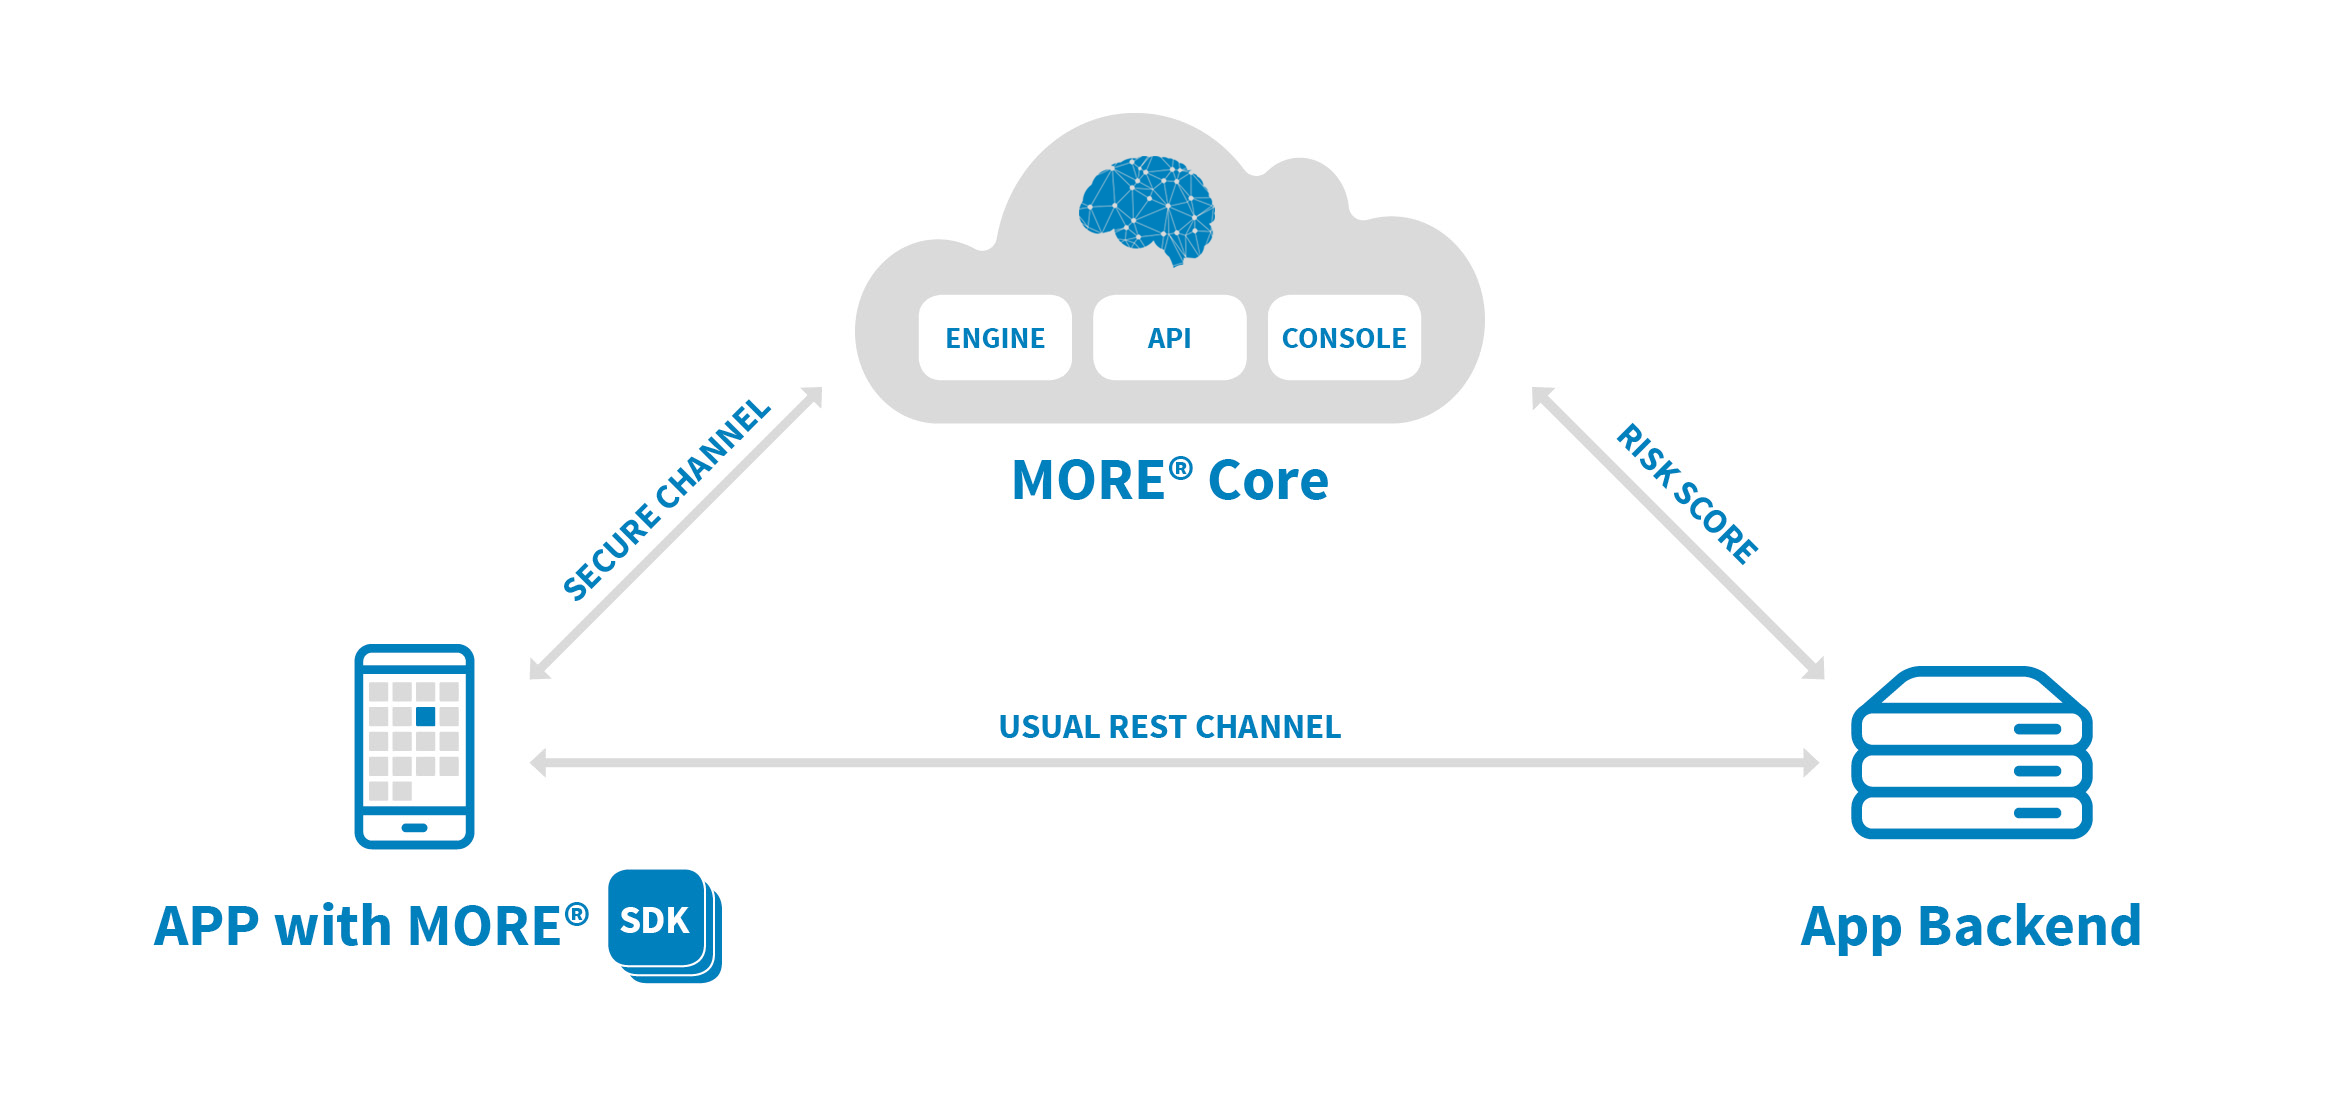
\includegraphics[scale=0.15]{immagini/more-arc.png}
	\caption{\textit{Architettura cloud More\textregistered} (\link{https://xtn-lab.com/more/})}
\end{figure}
\newpage
\section{Organizzazione aziendale}
XTN adotta l'\textit{Agile Team Organisation} tramite \textit{Squads, Chapters, Guilds}.
\begin{figure}[ht]
	\centering
	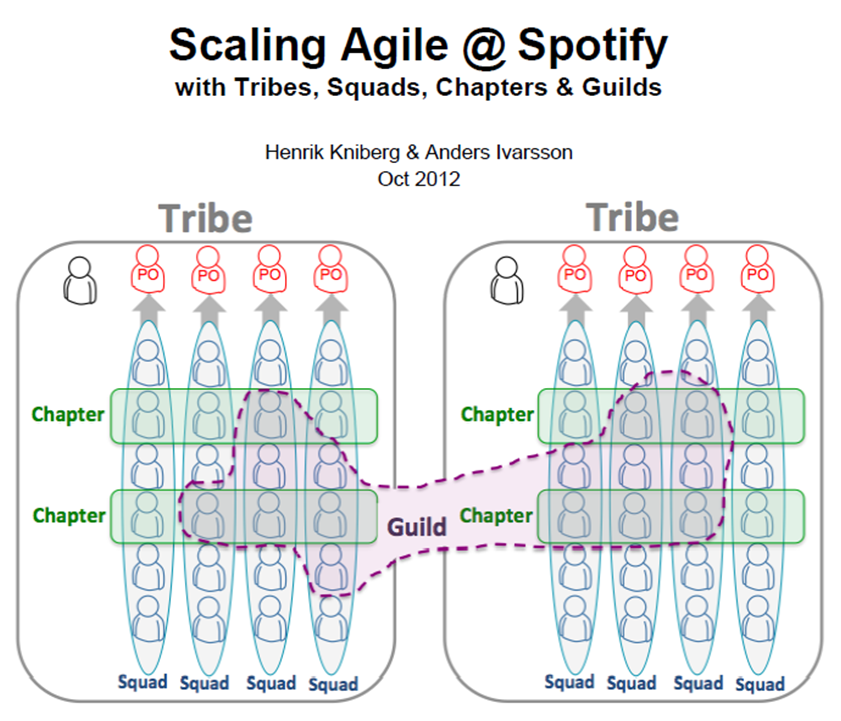
\includegraphics[scale=0.6]{immagini/agile-org.png}
	\caption{\textit{Agile Team Organisation (\link{https://goo.gl/fjJOO6}})}
\end{figure}
\begin{itemize}
\item{\textbf{Squads}:} sono un gruppo di persone che condividono il luogo di lavoro ed il campo di interesse. In XTN esistono due squads, uno per  Smash\textregistered\ ed uno per More\textregistered. Ogni squads si riunisce periodicamente, circa ogni settimana, per tracciare e discutere la situazione delle varie \textit{milestone}. 
\item{\textbf{Chapters}:} sono un gruppo di persone che condividono le competenze, trasversalmente ai vari squads, per promuovere l'innovazione e la collaborazione. Periodicamente, circa ogni mese, i vari chapters si riuniscono per convidivere informazioni di interesse e favorire un allineamento tecnologico tra i vari squads.
\item{\textbf{Guilds}:} sono una comunità di membri, in tutta l'organizzazione, che vogliono condividere conoscenze, strumenti e pratiche comuni. Ad esempio, in XTN, esiste una \textit{guild} nata per accrescere la conoscenza sull'intelligenza artificiale.
\item{\textbf{Tribe}:} sono nate per suddividere, e rendere piu gestibile, una grande infrastruttura. XTN non ha addottato questo concetto essendo ancora un azienda di piccole dimensioni.
\end{itemize}
In particolare, durante il periodo di stage, sono stato localizzato nello \textit{Squads} di Smash\textregistered\, ma non appartenevo a nessuna \textit{Guilds}.
\newpage

\section{Processi aziendali e strumenti di supporto}
In questa sezione verranno affrontati i processi aziendali e le tecnologie a supporto che ho avuto modo conoscere ed imparare lavorando a stretto contatto con il team di Smash\textregistered.

\subsection{Gestione della configurazione}
Tutti gli oggetti, che siano documentali e non, sono mantenuti in un repository interno. La configurazione è un insieme di questi oggetti che andranno a comporre una determinata versione del prodotto. Ogni configurazione ha il proprio identificativo univoco e un documento contenente informazioni utili all'istallazione del prodotto.\\
Ogni oggetto per essere aggiunto ad una determinata configurazione deve essere prima verificato dall'amministratore di progetto.
\subsubsection{Strumenti di supporto}
Per tener traccia di tutte le modifiche ed evitare sovrascritture involontarie l'azienda ha deciso di adottare una repository interna chiamata Stash. Quest'ultima è un sistema di gestione di repository che utilizza diversi sistemi di controllo di versione, tra cui Git e Mercurial. Infine l'azienda ha deciso di utilizzare Git come controllo di versione.
\subsection{Processo di sviluppo}
L'azienda si ritrova spesso a dover vendere il proprio prodotto con un certo numero di personalizzazioni. Per far ciò gli addetti alla vendita di XTN effettuano incontri con i clienti per ricavare idee ed osservazioni per, successivamente, stilarli in un documento. Questo documento poi verrà usato dal team di sviluppo per creare il prodotto in linea con le richieste del cliente.\\
L'azienda non rilascia protipi incompleti al cliente ma solamente prodotti funzionanti con tutte le personalizzazioni richieste.\\
Attualmente per ogni personalizzazione richiesta dal cliente il team di sviluppo cerca di renderla una \textit{feauture} usabile da tutti e quindi rivendibile.
\subsubsection{Strumenti di supporto}
\begin{itemize}
\item{\textbf{Backend}}\\
Per quanto riguarda la parte logica l'azienda ha deciso di utilizzare principalmente Java come linguaggio, in quanto è molto performante ed ha una sintassi molto regolare. Per quest'ultimo il team di sviluppo ha deciso di adottare il \textit{framework Spring} per astrarre, e semplificare, buona parte di architettura di \textit{backend}.\\
Per quanto riguarda la persistenza dei dati, XTN, ha deciso di adottare MongoDB.
\begin{figure}[ht]
	\centering
	
\includegraphics[scale=0.15]{immagini/java-spring.png}
	\caption{\textit{Logo Java e Spring (\link{https://goo.gl/Gm7usK})}}
\end{figure}
\item{\textbf{Frontend}}\\
Per quanto riguarda l'interfaccia grafica della \textit{dashboard} di Smash\textregistered, XTN ha deciso di adottare il \textit{framework AngularJS 1}. Quest'ultimo è sviluppato da Google e permette di semplificare lo sviluppo e \textit{test} di applicazioni web \textit{single page}.
\begin{figure}[ht]
	\centering
	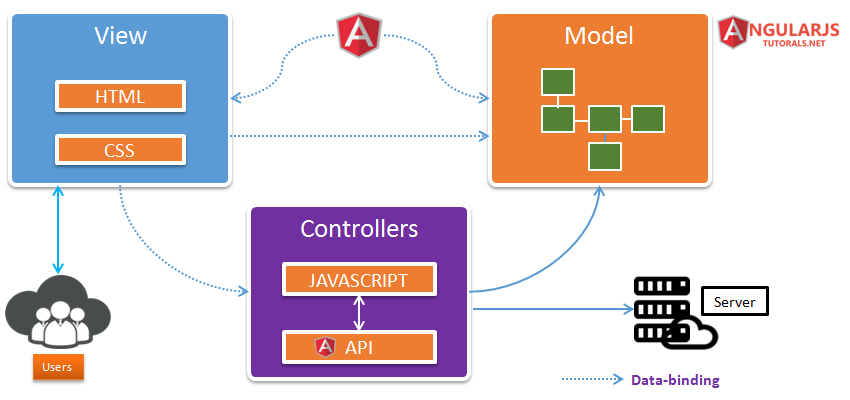
\includegraphics[scale=0.3]{immagini/angular.png}
	\caption{\textit{Architettura AngularJS (\link{https://goo.gl/PzB2v8})}}
\end{figure}
\end{itemize}

\subsection{Processo di manutenzione}
Ogni mulfunzionamento viene segnalato e tracciato con la rispettiva priorità. Il personale addetto risolverà le varie segnalazioni in ordine di priorità e successivamente, dopo la sistemazione di un certo numero di malfunzionamenti, il \textit{project manager} rilascerà la nuova versione del prodotto.
\subsubsection{Strumenti di supporto}
Qualunque malfunzionamento viene segnalato e registrato in un sistema di tracciamento delle \textit{issues} chiamato Jira. Questo servizio permette di assegnare, per ogni \textit{issues}, una priorità, una scadenza e la versione con cui il malfunzionamento sarà sistemato. 
\subsection{Processo di verifica}
Il processo viene gestito dal \textit{chapter} che garantisce la qualità del prodotto offerto. Questo gruppo di persone esegue delle prove per garantire degli \textit{standards}, in ambito di usabilità e prestazioni. Una volta verificate le varie parti il prodotto potrà essere messo in produzione






\section{Rapporto con l'innovazione}
Attualmente i prodotti di \textit{\azienda} hanno raggiunto una maturità tale per cui il servizio che si promettono di offrire coincide con quello che offre realmente. L'azienda, però, continua periodicamete ad investire risorse per trovare nuove tecnologie o soluzioni al fine di offrire un servizio sempre migliore.\\
Queste risorse vengono divise tra studi di settore per focalizzarsi sulle tecnologie del momento e, successivamente, vengono svolti progetti interni, come stage universitari, per verificare la fattibilità della soluzione in analisi. \\
Proprio a questo riguardo, da circa un anno, è in corso uno studio nella tecnologia di \textit{apprendimento automatico} attraverso corsi di formazione e convegni. Questo viene svolto per riuscire ad aggiungere funzionalità che permettono l'apprendimento automatico del comportamento abituale di determinati utenti. Aggiungere questa funzionalità permetterebbe di abbassare nettamente i falsi positivi di frode bancarie.


